% \begin{figure*}[t]
%     \centering
%     % 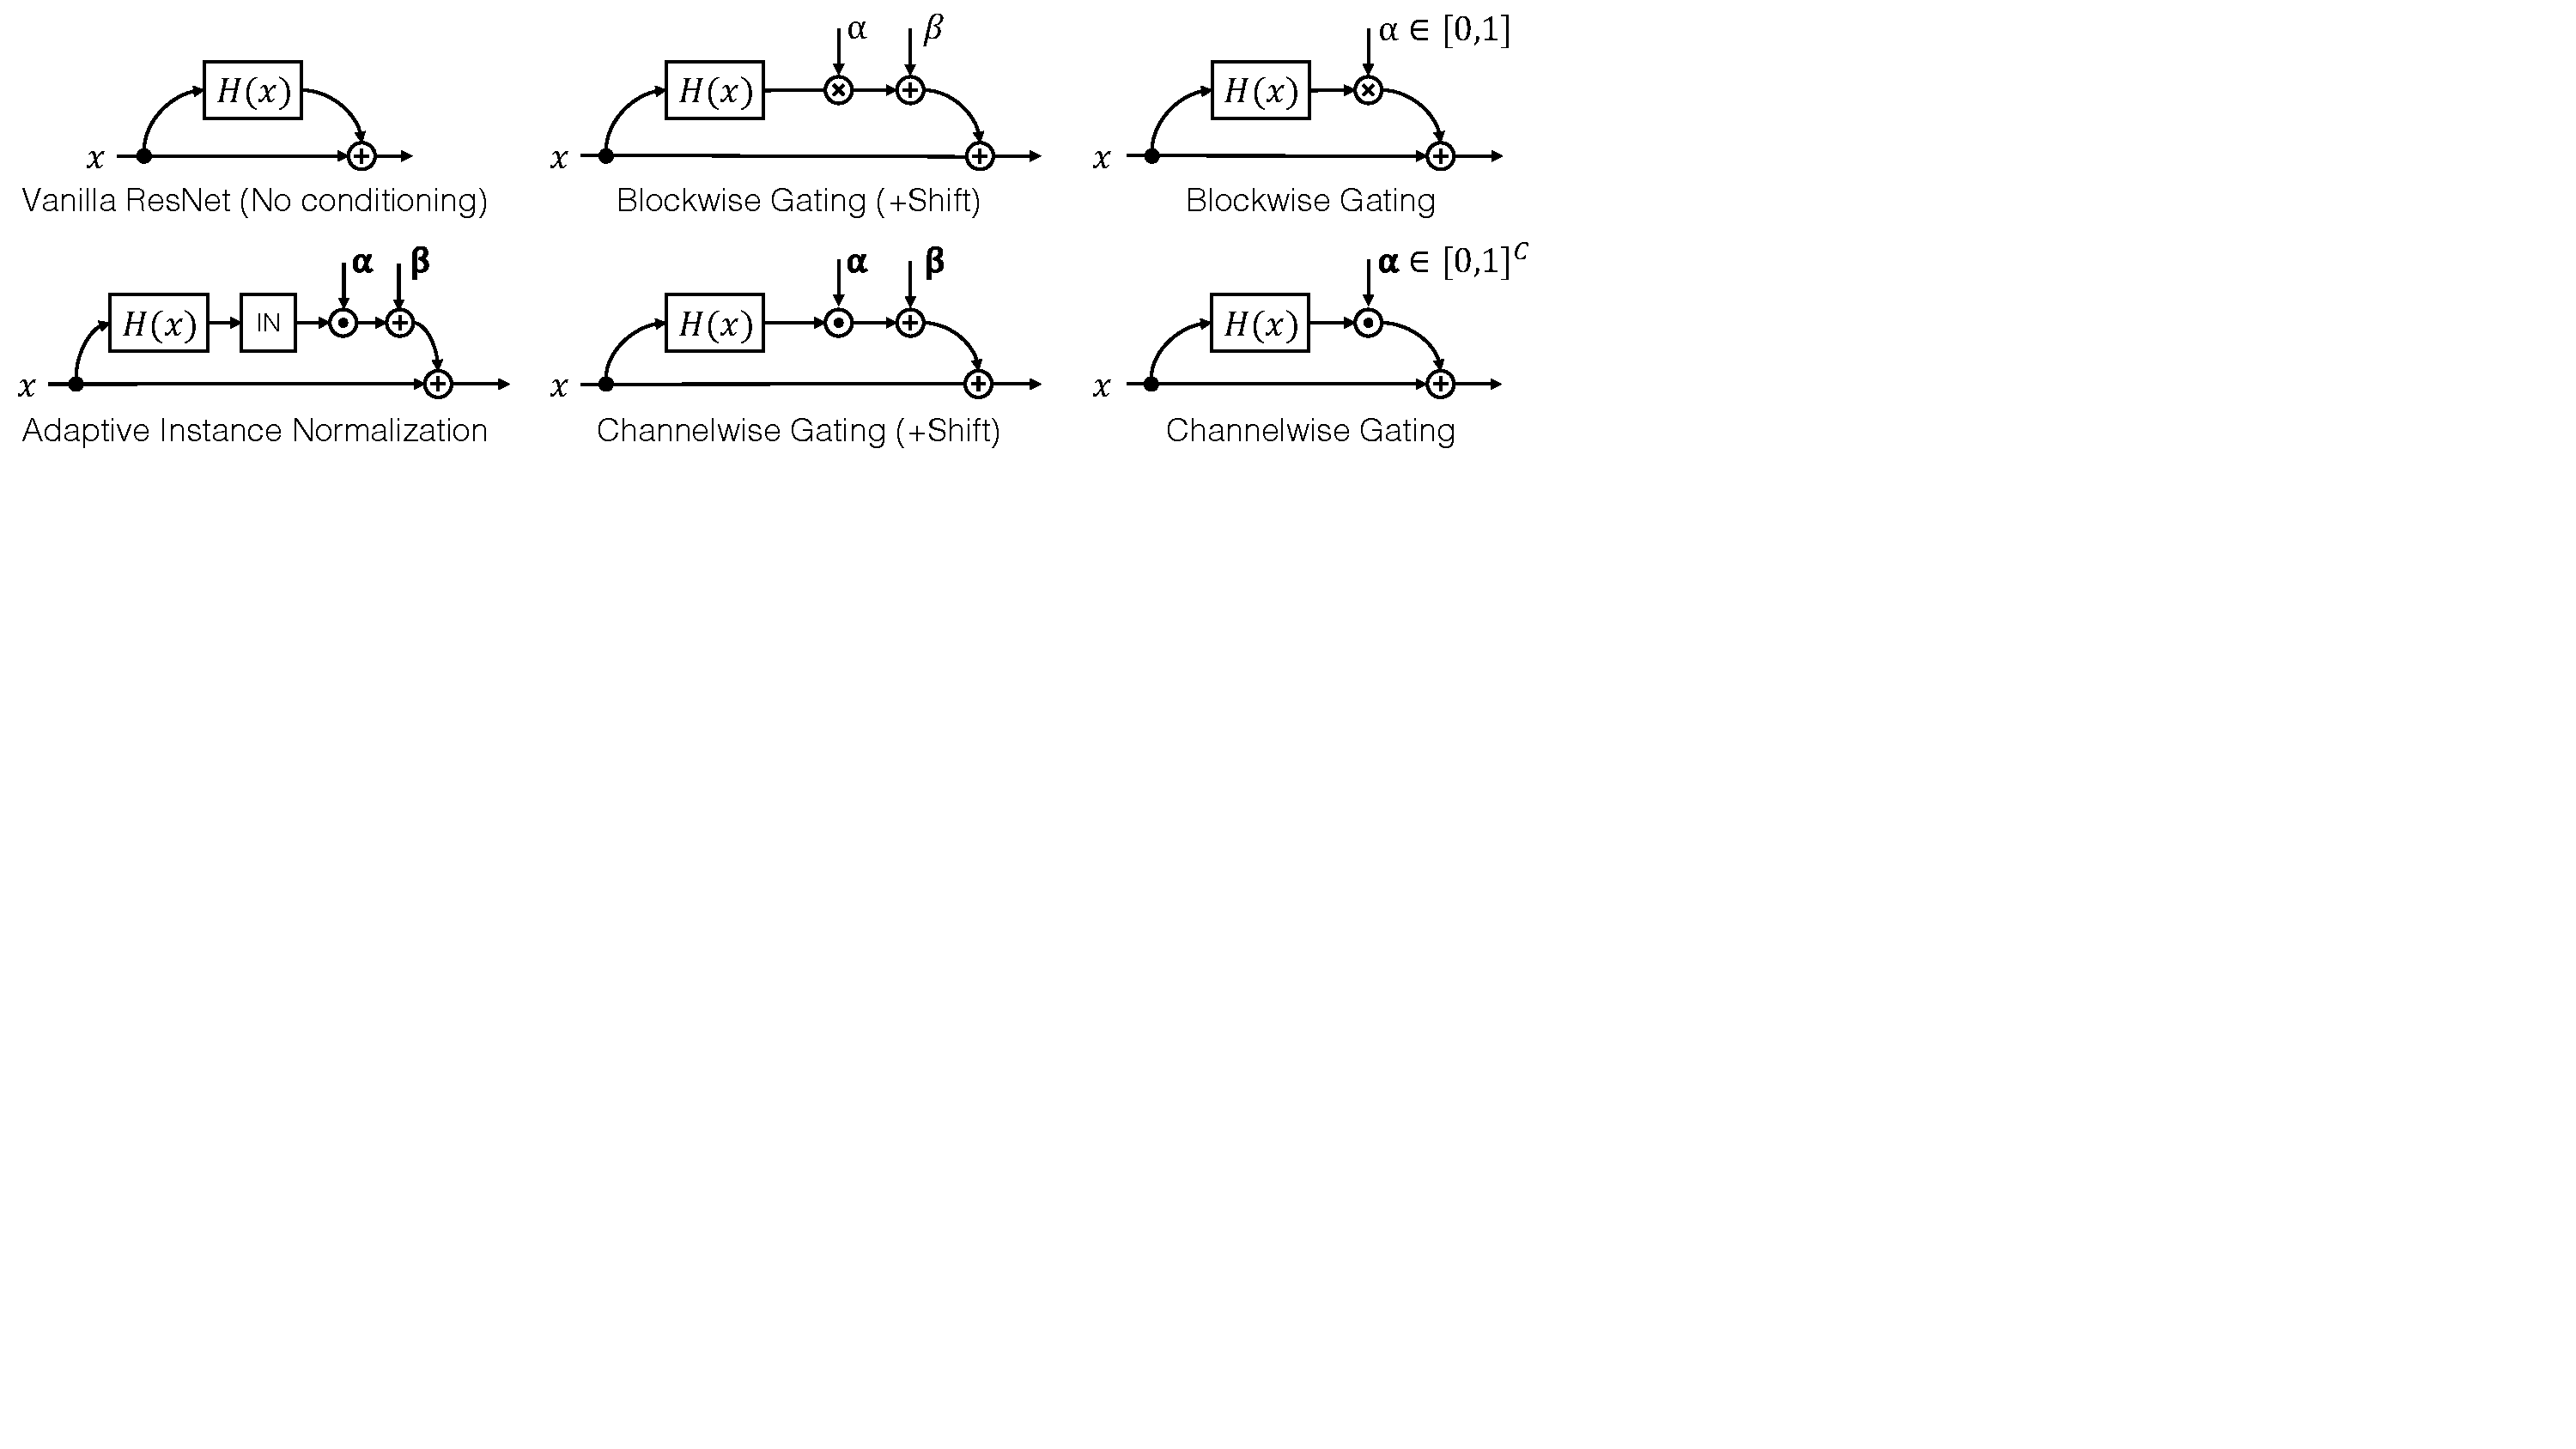
\includegraphics[width=\linewidth]{paper_images/arch_gate.pdf}
%     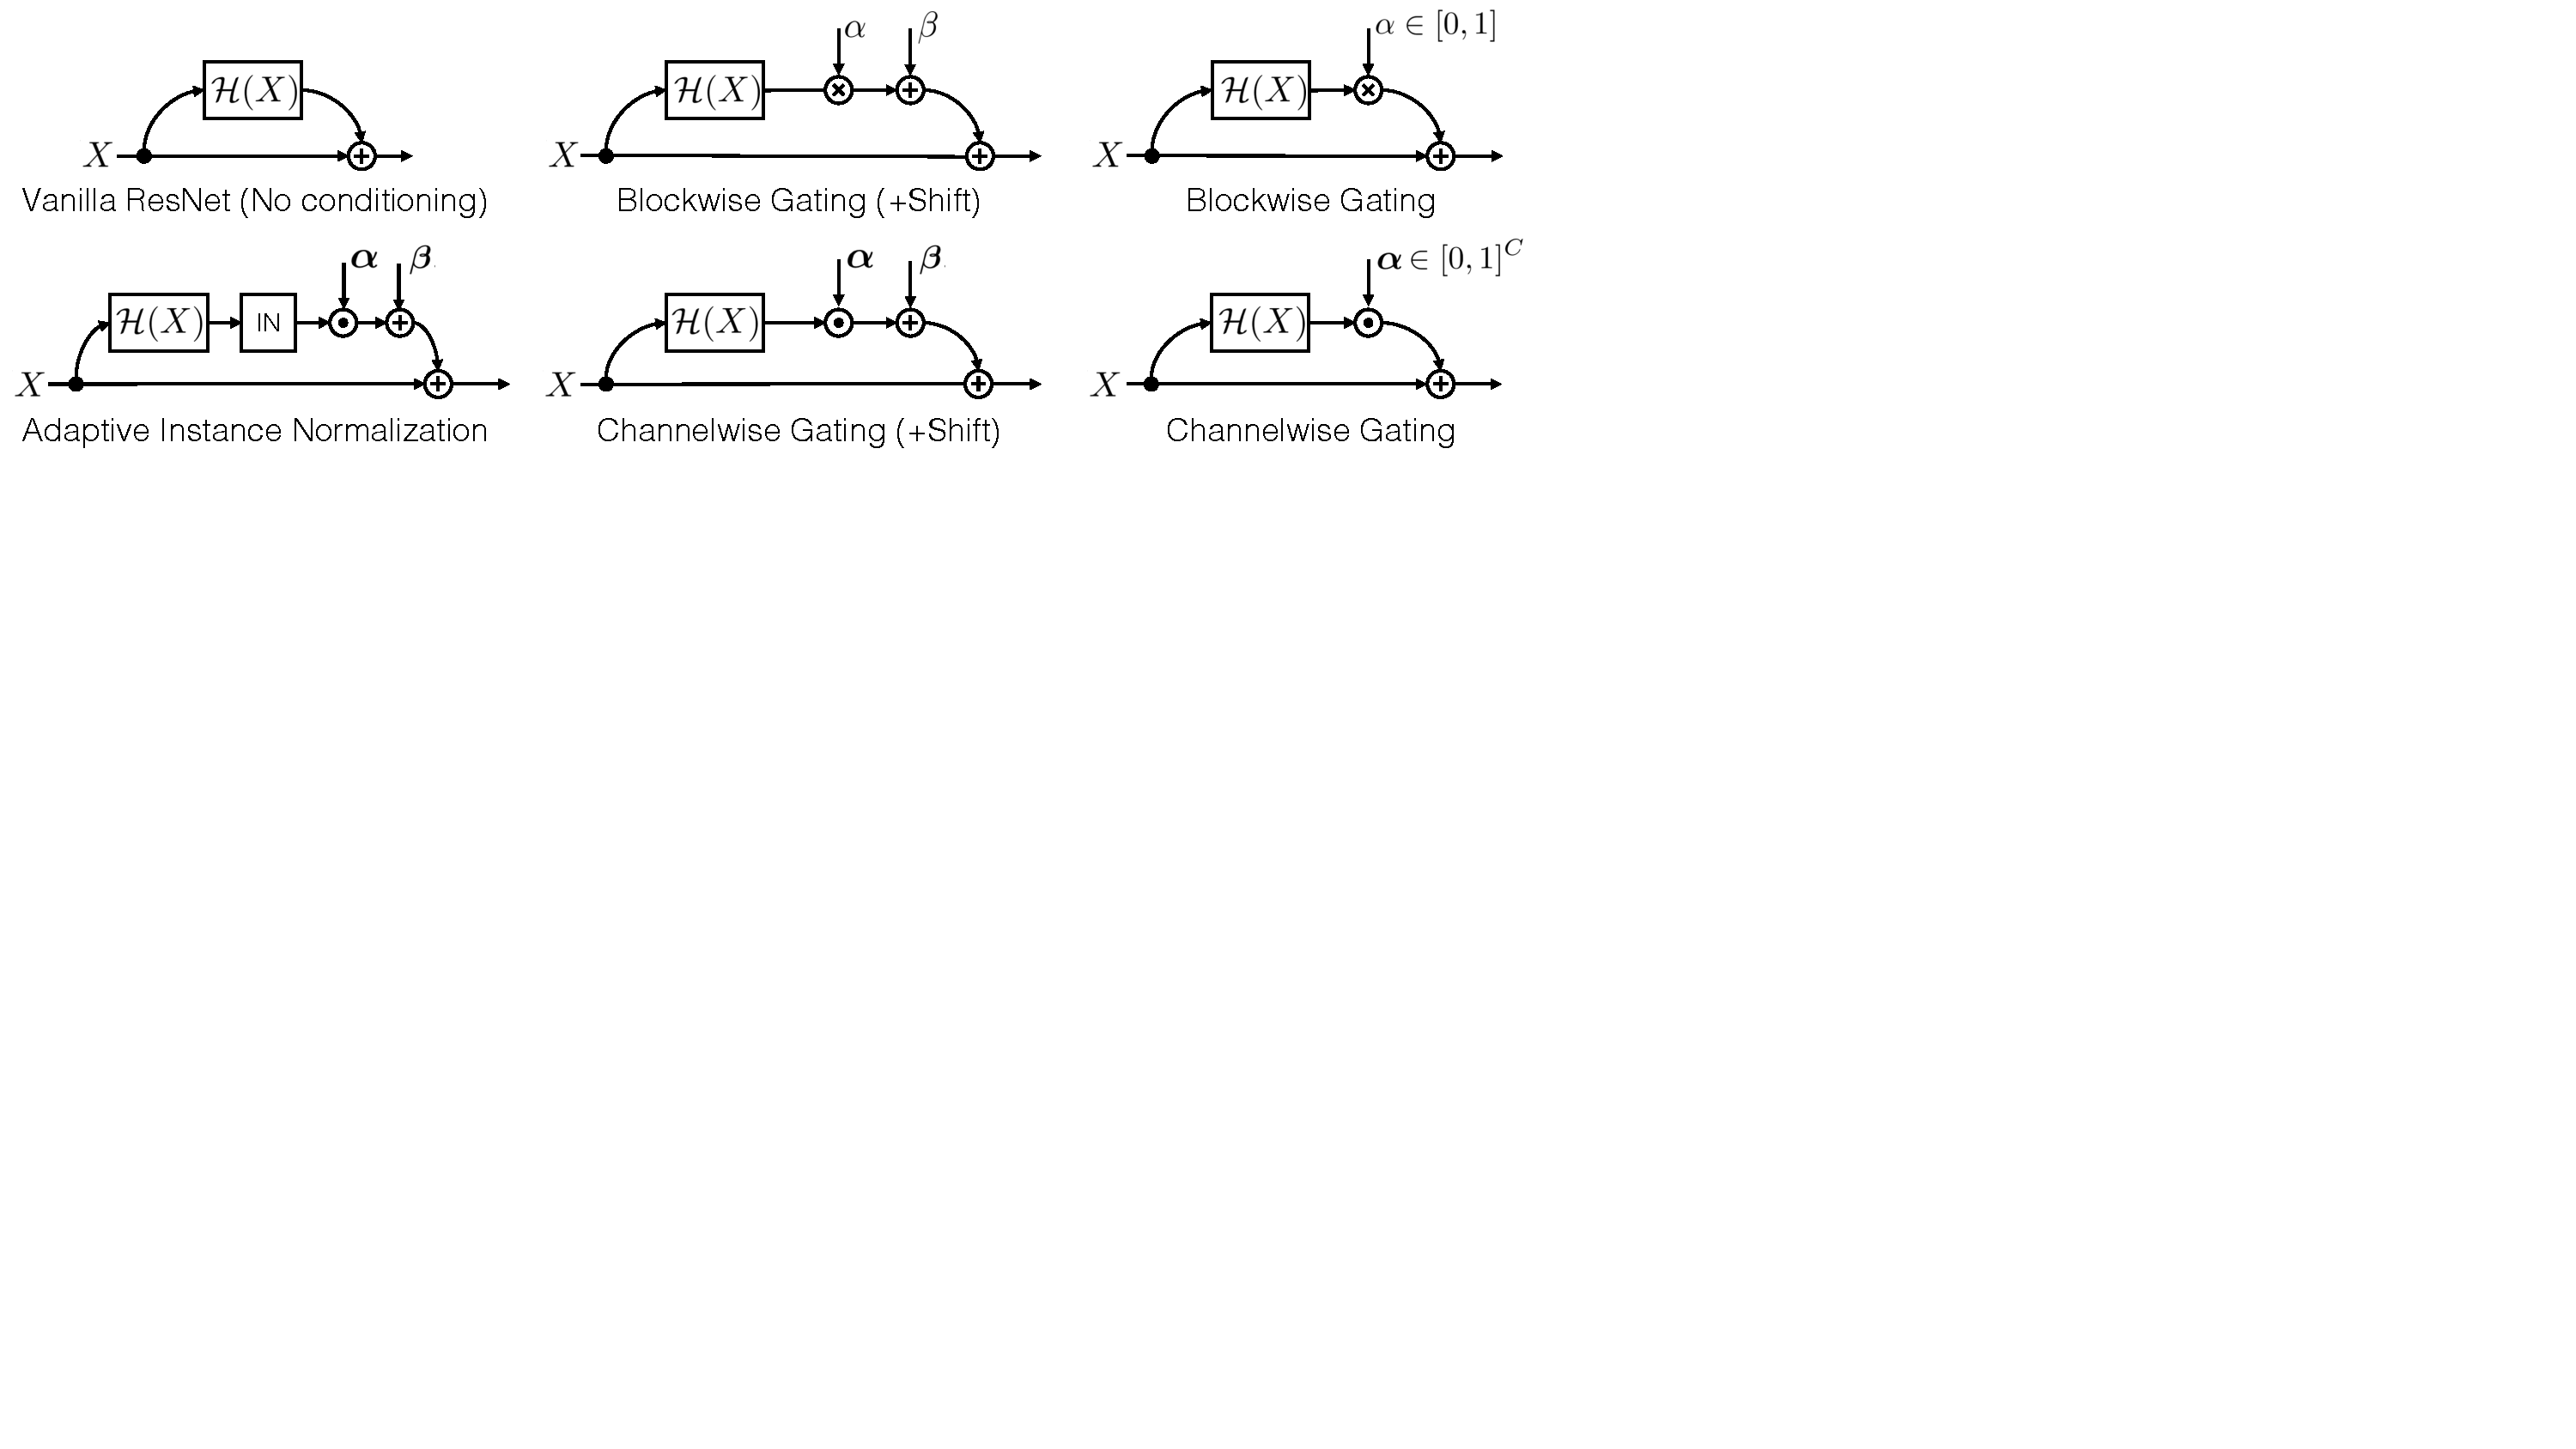
\includegraphics[width=.9\linewidth]{paper_images/arch_gate2.pdf}
%     \caption{
%     % {\bf Incorporating soft-gating into residual blocks.} \rz{Order got changed, may or may not need to add key for hadamard product}
%     {\bf (Top-left)} A ``vanilla" residual block without gated conditioning parameters modifies input tensor $X$ into $X+\mathcal{H}(X)$. Conditioning with concatenation uses this setup. {\bf (Top-mid)} The $\mathcal{H}(X)$ block is softly-gated by scalar parameter $\alpha$ and shift $\beta$. {\bf (Top-right)} Only the gating is used, without bias. {\bf (Bot-left)} Adaptive Instance Normalization~\cite{huang2017arbitrary} applies a channel-wise scaling and shifting after an instance normalization layer. {\bf (Bot-mid)} Channel-wise gating adds restrictions to the range of $\mbox{\boldmath $\alpha$}$. {\bf (Bot-right)} We find that channel-wise gating (without added bias) to empirically produce the best results.\label{fig:arch-gate}
%     \vspace{-2mm}
%     }
%     % \vspace{-4mm}
% \end{figure*}


% \begin{figure*}[t]
%     \centering  
%     \begin{tabular}{cc}
%     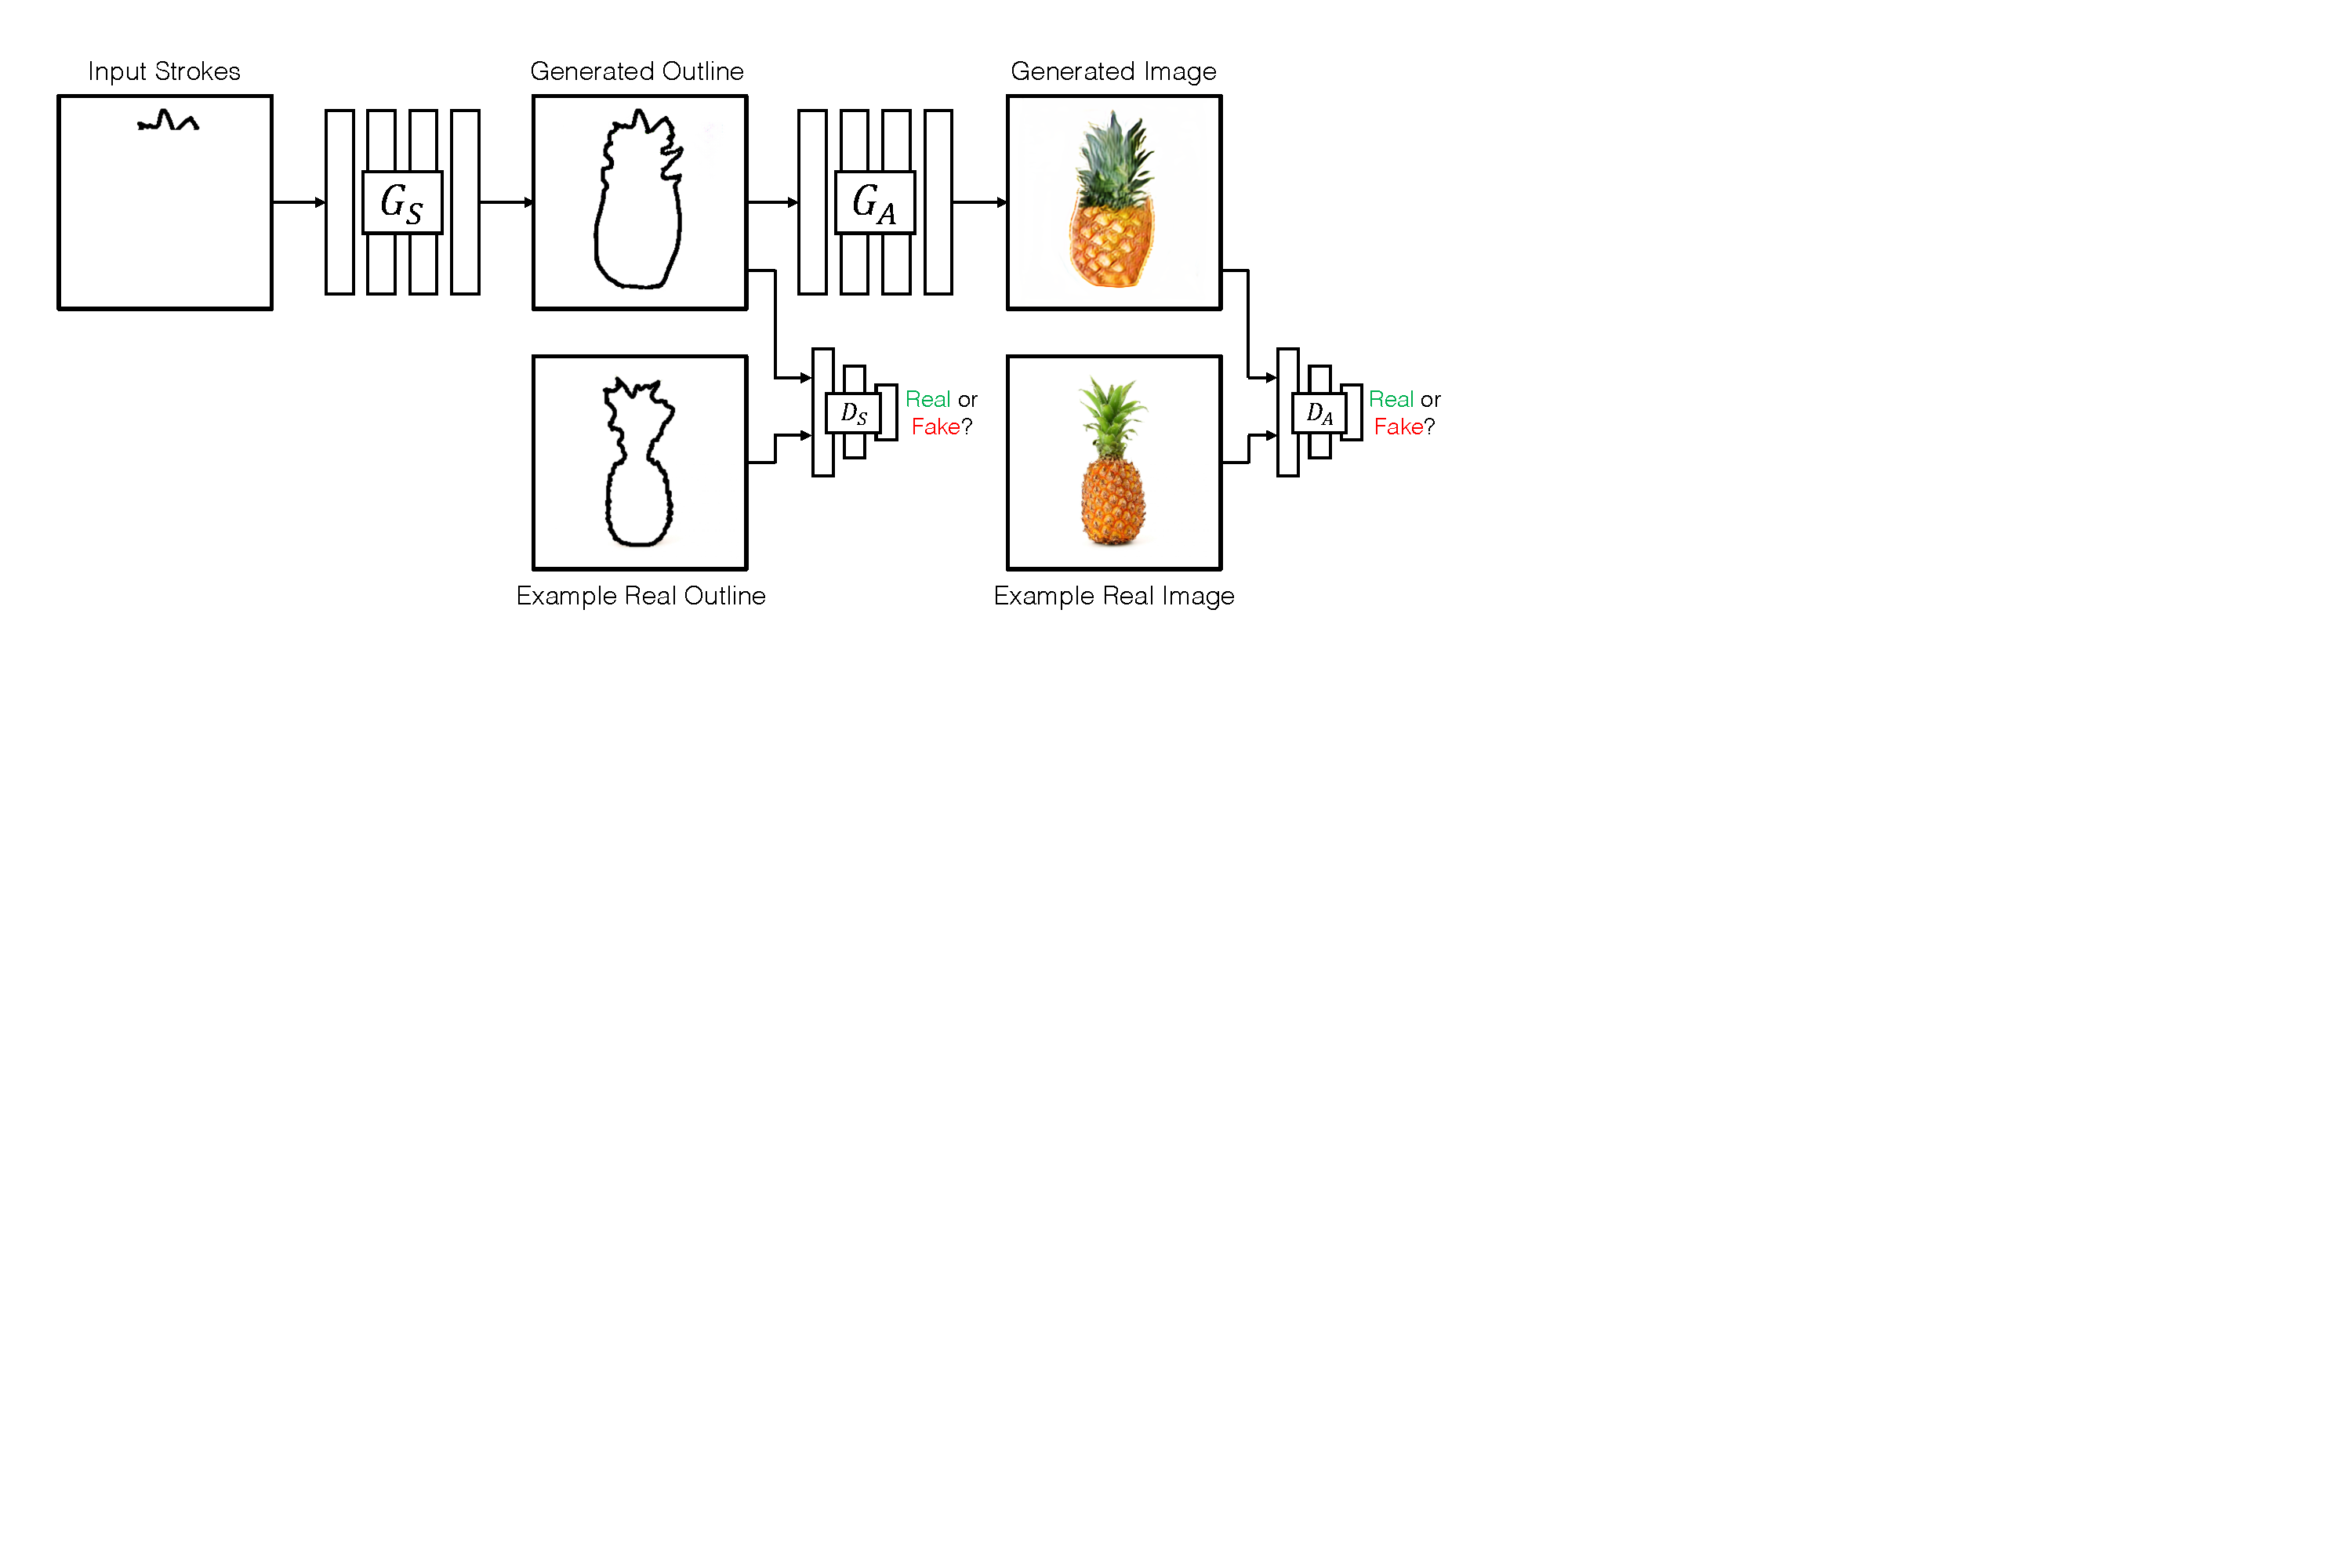
\includegraphics[width=.45\linewidth]{paper_images/isf_method_v3.pdf} &
%     \animategraphics[autoplay,loop,width=.45\linewidth]{25}{images/gif/}{00001}{00266}
%     \\
%     (a) & (b) \\
%     \end{tabular}
%         \caption{{\bf Our two-stage approach (a)} First, we complete a sketch, using the shape generator $G_S$. The appearance generator $G_A$ then translates the result into an image. Both generators are trained with respective discriminators $D_S$, $D_A$.
%         {\textbf{Video of our interface (b).} Please view with Acrobat Reader.}}\label{fig:SketchFillNet}
%         %\label{fig:gui}}
% \end{figure*}


% \begin{figure*}[t]
%     \centering  
%     \begin{tabular}{cc}
%     %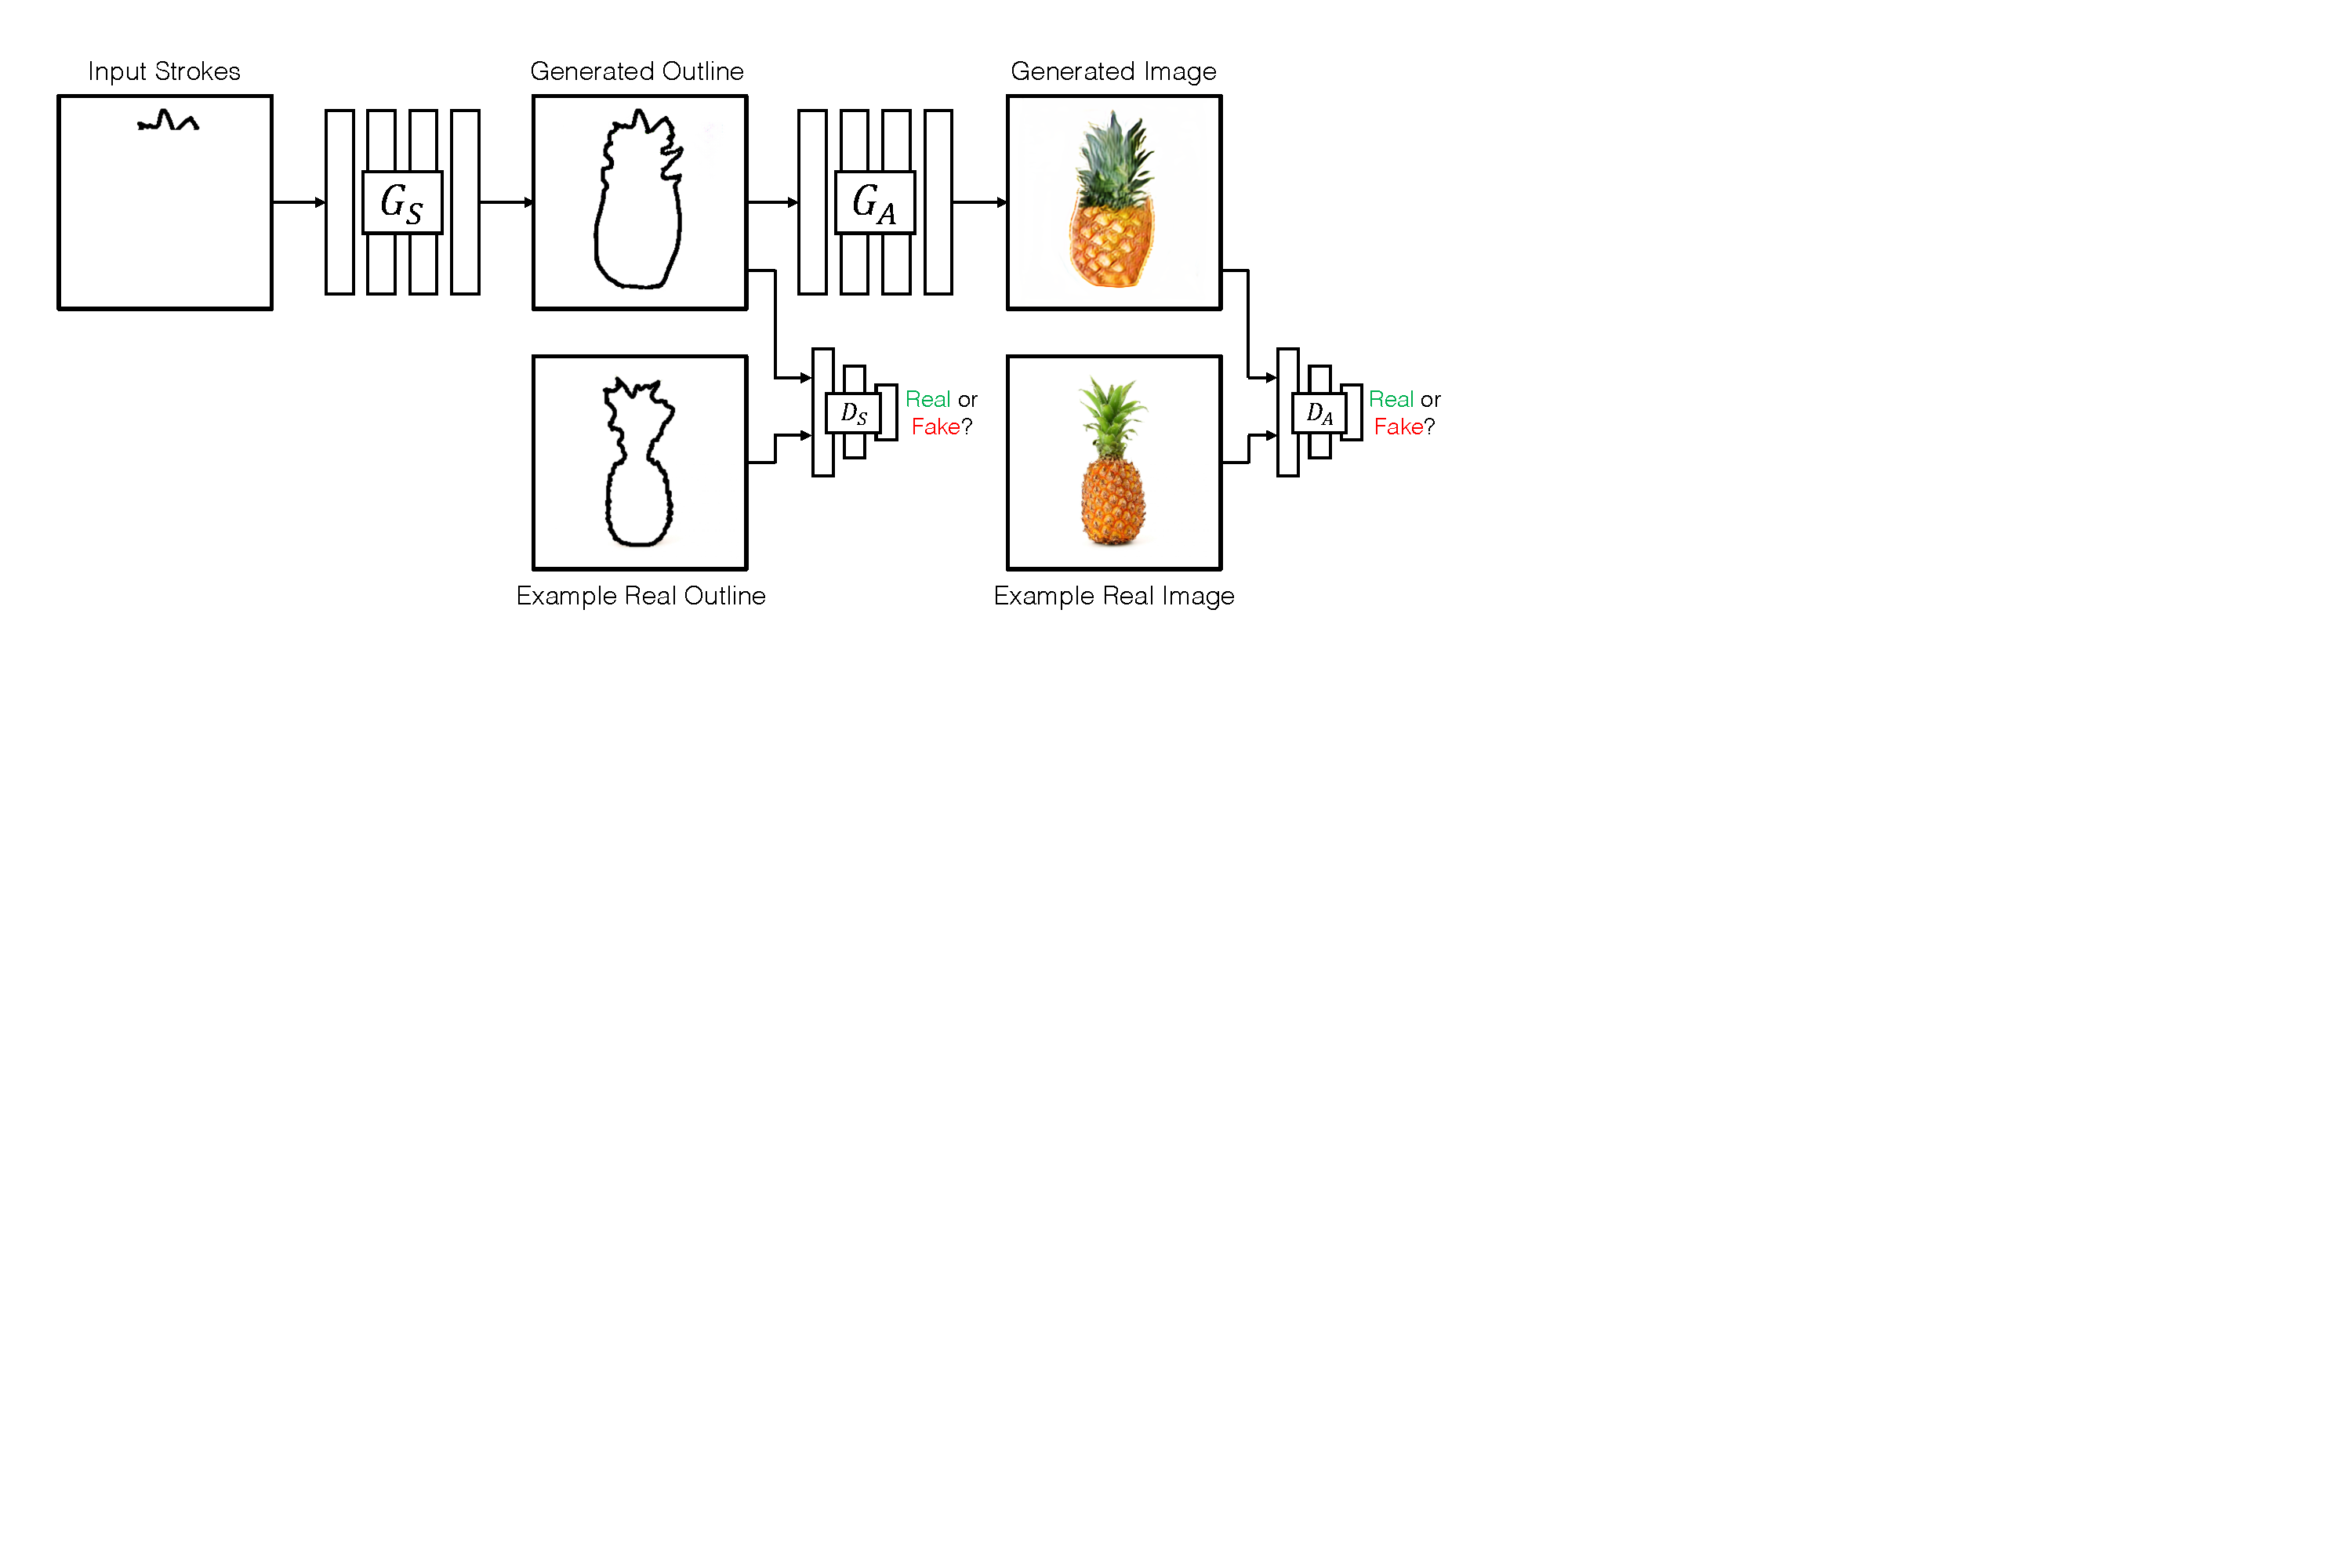
\includegraphics[width=.45\linewidth]{paper_images/isf_method_v3.pdf} &
%     \animategraphics[autoplay,loop,width=.45\linewidth]{25}{images/gif/}{00001}{00266} \hspace{4pt}
%     \animategraphics[autoplay,loop,width=.50\linewidth]{25}{images/gif_shadow/}{00001}{00419}
%     \\
%     % (a) & (b) \\
%     \end{tabular}
%         \caption{{\bf Video of our interface} We can see two versions of our interface. The left side shows how a user can quickly generate multiple objects using a few strokes, while the right side shows the utility of multimodal completions where the user can quickly explore different possible shape generations while drawing.
%         { \textbf{Please view with Acrobat Reader.}}}\label{fig:gui}
%         %\label{fig:gui}}
% \end{figure*}

\begin{figure*}[t]
    \centering  
    \begin{tabular}{cc}
    %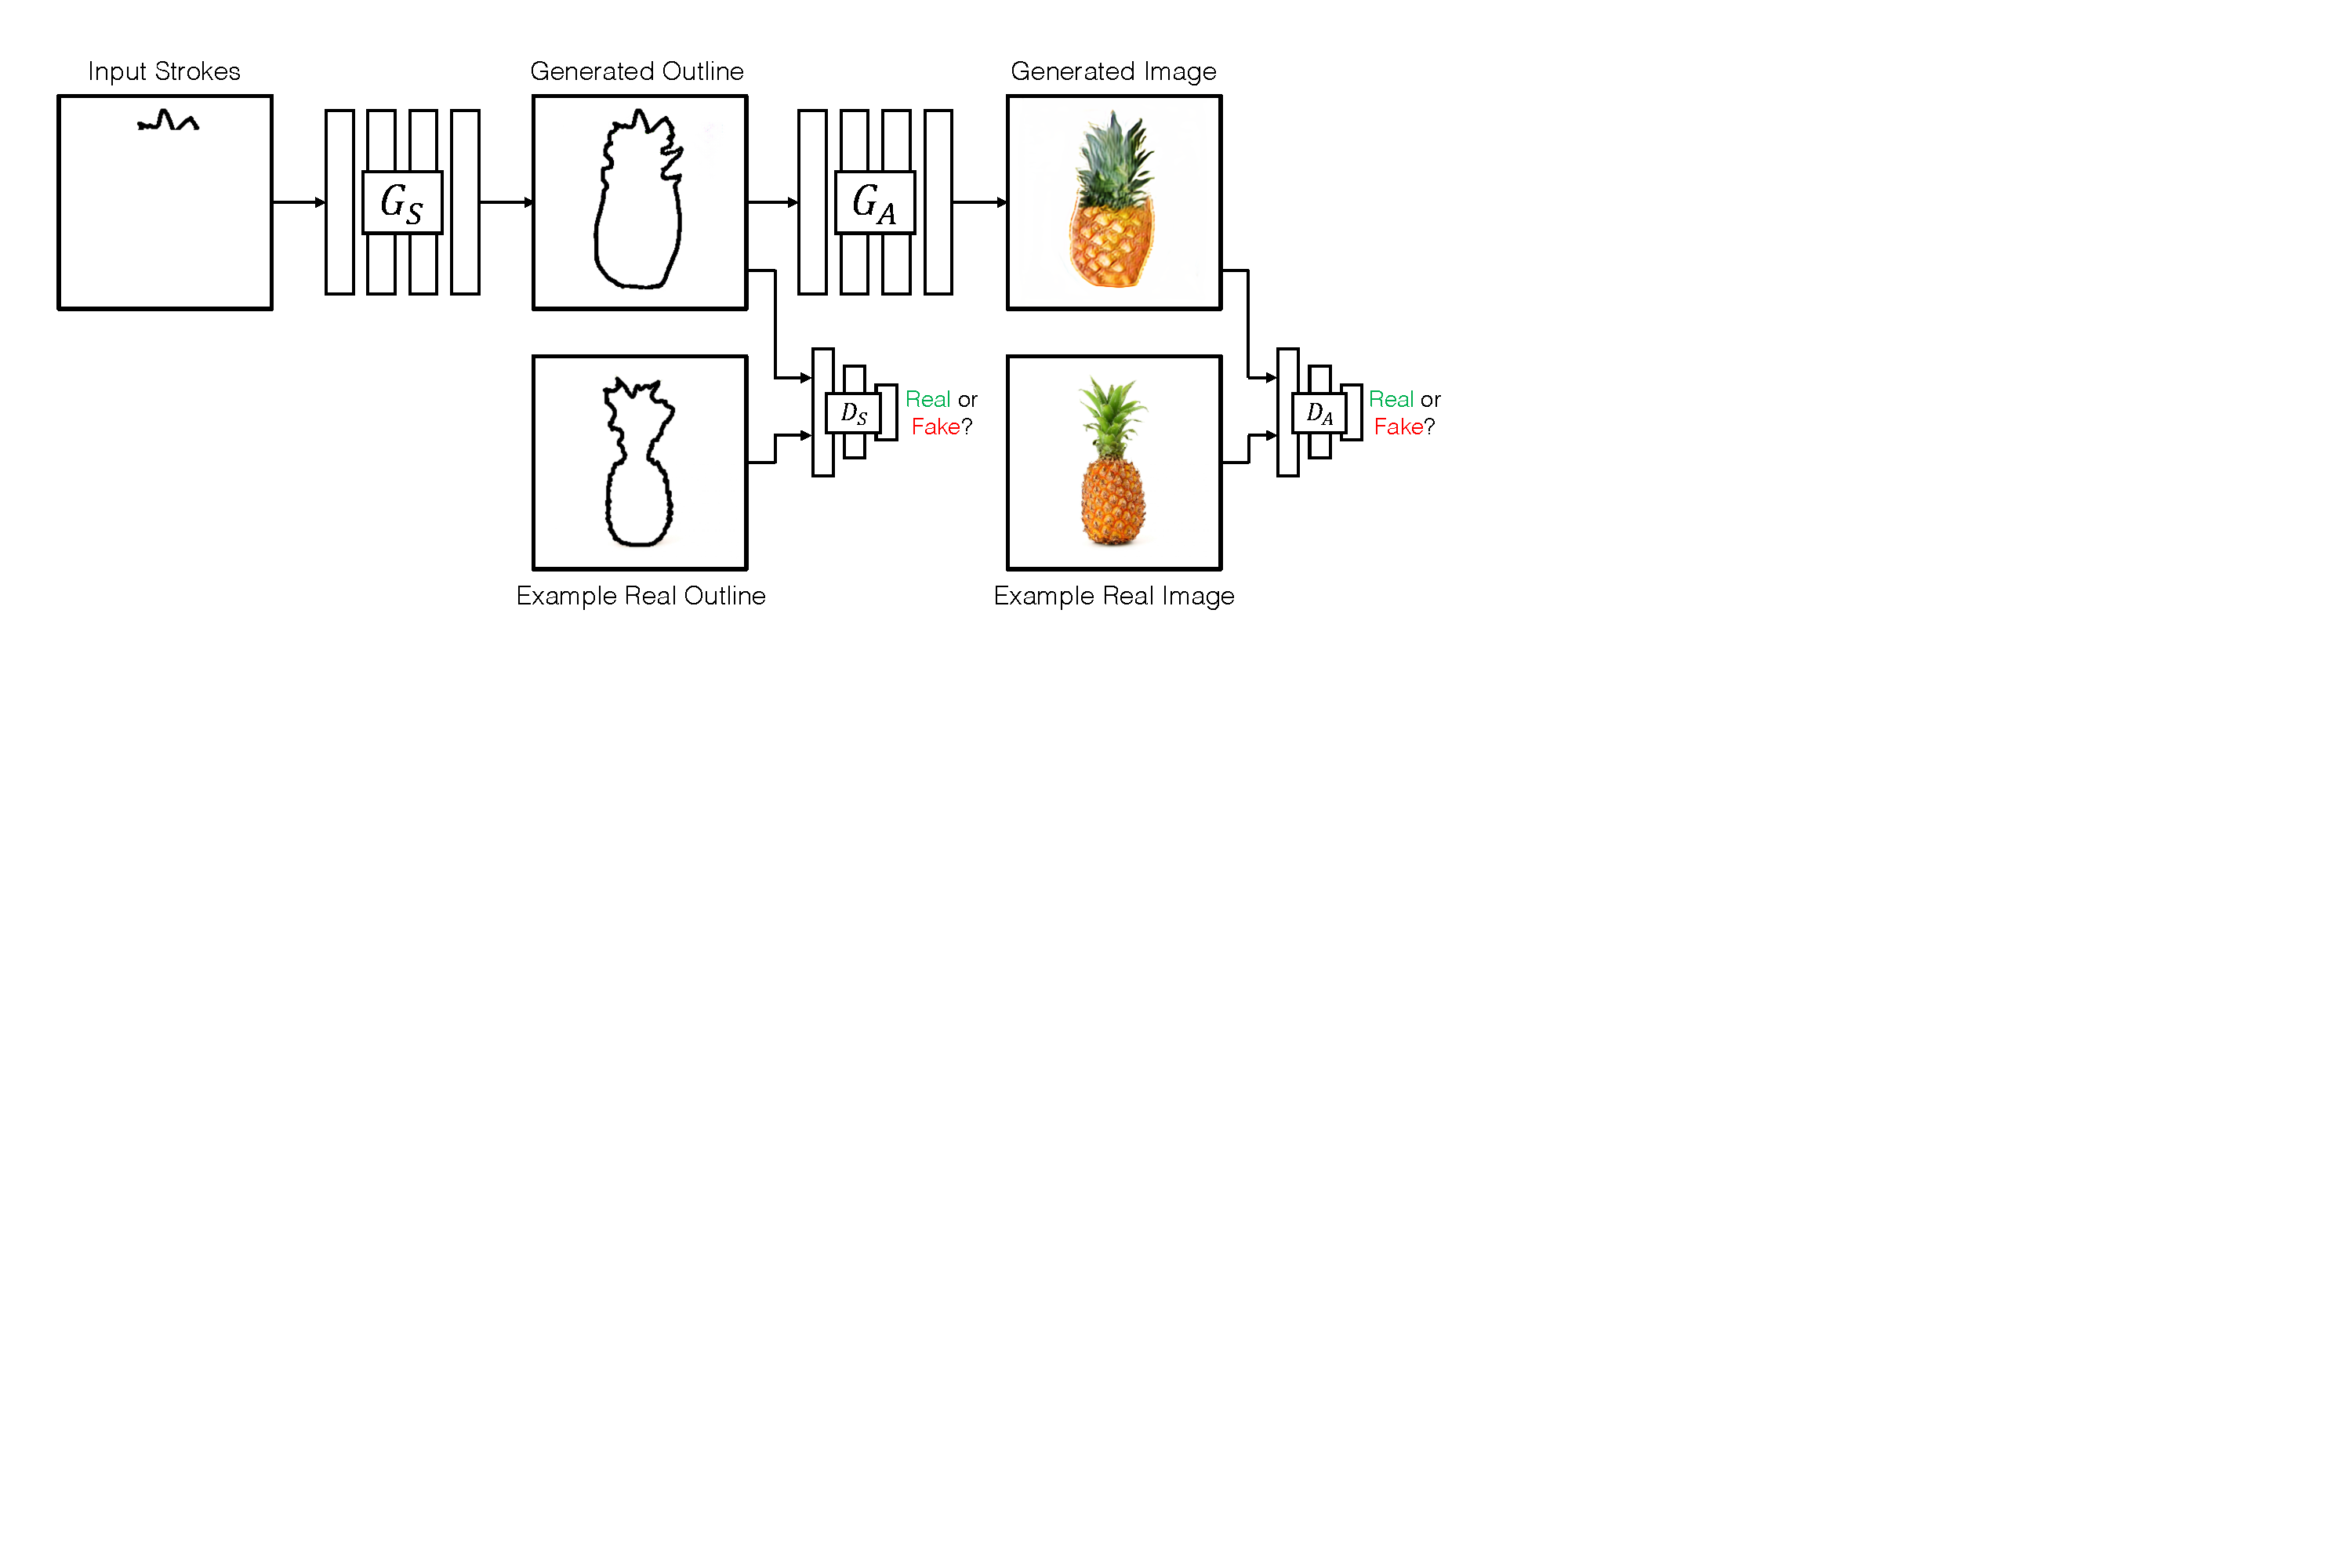
\includegraphics[width=.45\linewidth]{paper_images/isf_method_v3.pdf} &
    %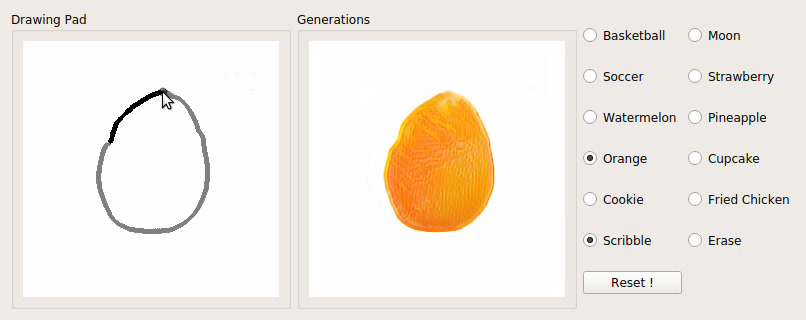
\includegraphics[width=.45\linewidth]{images/gif/00001.jpg} \hspace{4pt}
    %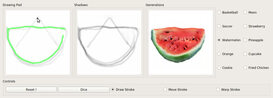
\includegraphics[width=.45\linewidth]{images/gif_shadow/00001.jpg} 
    \animategraphics[autoplay,loop,width=.45\linewidth]{25}{images/gif/}{00001}{00266} &
    \animategraphics[autoplay,loop,width=.50\linewidth]{25}{images/gif_shadow/}{00001}{00096}
    \\
    % (a) & (b) \\
    \end{tabular}
        \caption{{\bf Video of our interface} We can see two versions of our interface. The left side shows how a user can quickly generate multiple objects using a few strokes, while the right side shows the utility of multimodal completions where the user can quickly explore different possible shape generations while drawing. Full video available at our \href{https://arnabgho.github.io/iSketchNFill/}{website}. { \textbf{Please view with Acrobat Reader.}}}\label{fig:gui}
        %\label{fig:gui}}
\end{figure*}


\section{Related Work}

\paragraph{Interactive Generation} Interactive interfaces for freehand drawing go all the way back to Ivan Sutherland's Sketchpad~\cite{sutherland64}.  The pre-deep work most related to us, ShadowDraw~\cite{lee2011shadowdraw}, introduced the concept of generating multiple shadows for novice users to be able to draw sketches. PhotoSketcher \cite{eitz2011photosketcher} introduces a retrieval based method for obtaining real images from sketches. %Hays et al.~\cite{hays2007scene} introduce a retrieval-based method for filling scenes.
% \es{other old papers? Talk about ShadowDraw and other non-deep methods}. 
More recently, deep recurrent networks have been used to generate sketches~\cite{ha2017neural,ganin2018synthesizing}. Sketch-RNN~\cite{ha2017neural} provides a completion of partial strokes, with the advantage of intermediate stroke information via the Quickdraw dataset at training time. SPIRAL \cite{ganin2018synthesizing} learns to generate digits and faces using a reinforcement learning approach.
% to generate programs for synthesizing the final image.
Zhu et al.~\cite{zhu2016generative} train a generative model, and an optimization-based interface to generate possible images, given color or edge constraints. The technique is limited to a single class and does not propose a recommendation for the completion of the shape. SketchyGAN~\cite{chen2018sketchygan} also aimed at generating multi-class images but lacks interactive capability. In contrast to the above, our method provides interactive prediction of the shape and appearance to the user and supports multiple object classes.
% \vspace{-6mm}
\paragraph{Generative Modeling} Parametric modeling of an image distribution is a challenging problem. Classic approaches include autoencoders~\cite{hinton2006reducing,vincent2008extracting} and Boltzmann machines~\cite{smolensky1986information}. More modern approaches include autoregressive models~\cite{efros1999texture,van2016conditional}, variational autoencoders (VAEs)~\cite{kingma2013auto}, and generative adversarial networks (GANs). GANs and VAEs both learn mappings from a low-dimensional ``latent" code, sampled stochastically, to a high-dimensional image through a feedforward pass of a network. GANs have been successful recently~\cite{denton2015deep,radford2015unsupervised,arjovsky2017wgan}, and hybrid models feature both a learned mapping from image to latent space as well as adversarial training~\cite{donahue2016adversarial,dumoulin2016adversarially,larsen2016vaegan,chen2016infogan}.

% \vspace{2mm} 
\paragraph{Conditioned Image Generation} The methods described above can be conditioned, either by a low-dimensional vector (such as an object class, or noise vector), a high-dimensional image, or both. Isola et al.~\cite{isola2016image2image} propose ``pix2pix", establishing the general usefulness of conditional GANs for image-to-image translation tasks. However, they discover that obtaining multimodality by injecting a random noise vector is difficult, a result corroborated in~\cite{mathieu2015deep,pathak2016context,zhu2017toward}.
% introduced a set of tasks whereby the pixels of the input in a different domain corresponded to the pixels of the generated image.
% As a result, image-to-image translation methods have exploded in popularity, as many applications can be expressed in this framework.
% However, one problem with the original Pix2pix formulation is that the quality degrades quickly with increased class diversity. 
% We build upon these ideas by proposing a new architecture and gating scheme that allows for high quality multiclass image generation. 
% \paragraph{Mode Collapse}
This is an example of mode collapse~\cite{goodfellow2016nips}, a phenomenon especially prevalent in image-to-image GANs, as the generator tends or ignore the low-dimensional latent code in favor of the high-dimensional image.
% This is an example of mode collapse is a major challenge for GANs~\cite{goodfellow2016nips}, where the diversity of the generated results is limited and only a portion of the training set is utilized. 
Proposed solutions include layers which better condition the optimization, such as Spectral Normalization~\cite{zhang2018self,miyato2018spectral}, modifications to the loss function, such as WGAN~\cite{arjovsky2017wasserstein,gulrajani2017improved} or optimization procedure~\cite{heusel2017gans}, or modeling proposals, such as MAD-GAN~\cite{ghosh2017multi} and MUNIT~\cite{huang2018multimodal}. 
% Several techniques deal with this issue, the best performing among those include Spectral Normalization \cite{zhang2018self,miyato2018spectral} which normalizes the spectral norms of the layers to stabilize training, MAD-GAN \cite{ghosh2017multi} which introduces multiple generators, BicycleGAN \cite{zhu2017toward} which reconstructs the latent code from the generation using two cycles, and MUNIT \cite{huang2018multimodal} which introduces a factorized latent space for content and style for producing variations.
One modeling approach is to add a predictor from the output to the conditioner, to discourage the model from ignoring the conditioner. This has been explored in the classification setting in Auxiliary-Classifier GAN (ACGAN)~\cite{odena2016conditional} and regression setting with InfoGAN~\cite{chen2016infogan} and ALI/BiGAN (``latent regressor" model)~\cite{dumoulin2016adversarially,donahue2016adversarial}, and is one half of BicycleGAN model~\cite{zhu2017toward}. We explore a complementary approach of architectural modification via gating.

% \ow{not clear to me why it starts with mode collapse... dangerous as we also have it in our results, except the infogan case. I think that this should be changed into an infogan related work section and moved below.}

%but needed far more details such as in the case of edge to handbags generation task it needed texture strokes inside the bag as well to be able to produce high quality diverse generations
%Other forms of conditioning have been introduced in \cite{wang2018video} whereby rough triangles and sparse edges are enough to generate high quality videos. We explore the situation in which the input scribble is extremely sparse and multiple classes can have very similar input scribbles for instance in the case of balls the input scribble is just the outline in the shape of a circle.

%Our architecture also differs from previous art in the form of the architecture whereby all the blocks are residual including the downsampling and upsampling. Previous literature mostly used the residual blocks in the bottleneck layer of an Encoder Decoder structure. The number of channels in the networks doesn't change with the change of resolution as in the original Resnet architecture \cite{he2016deep} in order to ease the learning of the gating mechanism. 

% \vspace{2mm} 
\noindent \textbf{Gating Mechanisms}
%Residual Networks \cite{he2016deep} introduced a new set of architectures that enabled training of very deep networks.
Residual networks~\cite{he2016deep}, first introduced for image classification~\cite{krizhevsky2012imagenet}, have made extremely deep networks viable to train. Veit et al.~\cite{veit2016residual} find that the skip connection in the architecture enables test-time removal of blocks. Follow-up work~\cite{veit2018adaptive} builds in block removal during training time, with the goal of subsets of blocks specializing to different categories. Inspired by these results, we propose the use of gating for image generation and provide a systematic analysis of gating mechanisms.
% Prior work has demonstrated that in ResNets, some paths are more important for particular classes~\cite{veit2016residual}, and has used this to develop a hard gating mechanism~\cite{veit2018adaptive}.
% We provide a further analysis of gating mechanisms, in the context of GAN image generation, as opposed to image classification.

The adaptive instance normalization (AdaIn) layer has similarly been used in arbitrary style transfer~\cite{huang2017arbitrary} and image-to-image translation~\cite{huang2018multimodal}, and Feature-wise Linear Modulation (FiLM)~\cite{perez2017film}. Both methods scale and shift feature distributions, based on a high-dimensional conditioner, such as an image or natural language question. Gating also plays an important role in sequential models for natural language processing: LSTMs \cite{hochreiter1997long} and GRU \cite{cho2014learning}. Similarly, concurrent work \cite{karras2018style}, \cite{park2019semantic} use a AdaIN-style network to modulate the generator parameters.
% \es{Mention concurrent work? StyleGAN, Taesung's paper}

% Our approach is related to adaptive instance normalization (AdaIn) has been used to great success in style transfer~\cite{huang2017arbitrary} and multimodal image-to-image translation~\cite{huang2018multimodal}.
% We use a fully residual architecture, and employ soft-gating both in the generator and discriminator. 
%Although previous work has explored the idea of gating via AdaIN in the generator but our techniques also involves using gating in the discriminator as well. 
% We evaluate AdaIn style gating among other possible choices with our architecture, and show that channel gating achieves superior performance for our task. Another gating mechanism, FiLM~\cite{perez2017film}, was introduced in the context of Visual Question Answering.
% In this case, the gating mechanism is conditioned on the input question.
% Gating also plays an important role in natural language processing: LSTMs \cite{hochreiter1997long} and GRU \cite{cho2014learning}.


% The seminal work by \cite{miyato2018spectral}, introduced spectral normalization which normalizes the weights of the network such that the maximum eigen value of the resulting set of weights is bounded. It helped enormously in stabilizing the training of GANs and albeit they only applied spectral normalization to the discriminator, SA-GAN \cite{zhang2018self} applied it to both the generator and discriminator and showed superior generative modeling performance over several tasks. SA-GAN further introduced the self attention layer based on the innovative transformer network and showed not only better geometric properties being modeled by the GAN but also allowing Multi-Class generations.
% The Projection Discriminator \cite{miyato2018cgans} based Conditional GANs altered the naive model of concatenating the condition provided to the discriminator via a generalized bilinear projection between the condition and the features extracted from the image thereby providing more finegrained gradients suitable for training the generator to produce class conditional and better resolution images. 
% MAD-GAN \cite{ghosh2017multi} introduced multiple generators and showed an innovative experiment whereby they mixed images from 3 classes and the 3 generators could disentangle the classes and each of the generators generated much sharper images from a particular class than a single generator with similar capacity could. 

% %moved from intro
% To combat this challenge a solution called MAD-GAN \cite{ghosh2017multi} was proposed which dealt with the issue via multiple generators whereby the discriminator distributed the modes and classes in the data distribution among the various generators. 
% Although MAD-GAN was a novel solution to deal with discontinuities in the manifold of the multi-class data distribution, the solution came with its flaws, supreme among them was the reduced scalability in the case the structure was not shared among the different classes, the generators couldn't share the initial layers' parameters and therefore was limited by GPU capacity and in practice going more than 5-6 generators was difficult. 

% In another line of papers which helped build the ideas in this paper are the research on Residual Networks \cite{he2016deep} which introduced a set of architectures which allowed extremely deep networks to be trained upto hundreds of layers which was earlier assumed to be extremely difficult because of the problem of vanishing gradients in deep networks. The residual connection allowed a unadulterated gradient backpropagation pathway which enabled training of ultra deep networks. A thorough analysis of residual networks by \cite{liao2016bridging} showed that residual networks have similar connections to unrolled recurrent neural networks without weight sharing and is very similar to how computation unfolds in human brains. Veit et al. \cite{veit2016residual} did a set of innovative incision experiments whereby they removed some blocks and allowed only the skip connection to be active in a trained Residual Network and they were able to demonstrate that even after removing some layers there a very miniscule reduction in the classification accuracy while a similar incision in a VGG network \cite{simonyan2014very} which doesn't have skip connections led to almost random outputs in the task of classification. \cite{veit2016residual} also demonstrated that residual networks behave as an ensemble of several shallower networks. \cite{veit2018adaptive} used the concepts introduced in \cite{veit2016residual} to introduce a discrete gating mechanism in deep residual networks based on the Gumbel-Softmax approximation to make the discrete decision differentiable. Their approach allowed redundant computations in the residual blocks to be reduced and to use only few of the blocks in the trained network during testing phase of the neural network. \cite{de2017modulating} introduced a technique for modulating the activations of a residual block by predicting the parameters of batch normalization which they term as Conditional Batch Normalization. In a similar vein \cite{perez2017film} also used a similar technique for modulating the activations of the various blocks conditioned on the question in a Visual Question Answering scenario.

% Gating mechanisms have generally been useful for language modeling tasks such as LSTMs \cite{Hochreiter1997LSTM} and \cite{chung2014empirical} which improved language modeling performance over vanilla RNNs. Gating also helped in the case of image recognition as demonstrated in Highway Networks \cite{srivastava2015highway} albeit it has a lot of resemblance to residual networks. 

% Image manipulation and Generation has seen huge strides in recent years with the advent of Generative Adversarial Networks \cite{goodfellow2014generative}, style transfer networks \cite{gatys2015neural} and image colorization \cite{zhang2016colorful}. iGAN \cite{zhu2016generative} was one of the first very innovative papers that introduced us to a novel technique for editing images using neural networks and preventing the edited images to fall off the natural image manifold. Pix2pix \cite{isola2016image2image} introduced a novel network based on GANs which could translate images on a plethora of datasets such as edges to handbags, semantic layout to photo realistic images and day to night. Cutting edge techniques on similar lines include \cite{wang2018video} which can translate from Video to Video such as from pose sequences to a person dancing or from semantic layouts to photorealistic road scenes. InfoGAN \cite{chen2016infogan} introduced a novel network based on GANs and Information Theoretic principles which could disentangle modes in the data distribution based on an unsupervised objective but showed poor performance in being able to disentangle modes and produce stochastic variations in the setting of pix2pix which is known to collapse to a single output for a particular input whereas ideally it should be a distribution. Bicycle GAN \cite{zhu2017toward} introduced 2 cycles which was able to produce stochastic generated outputs in the case of image to image translation. Another innovation was CycleGAN \cite{zhu2017unpaired} which allowed unpaired image to image translation as well as unpaired domain transfer which enabled several transformations which wasn't possible earlier. 

